\chapter{Team Model}\label{chapter:team_model}

When evaluating players, it is very important to realize that the team they play for and their opponent will have a strong influence on their performance no matter the skill level.
\textit{Find something that states a player is directly affected by their team}

\section{Dixon and Coles}
Dixon and Coles set out to create a model that incorporates team's attacking and defending abilities \cite{dixon_coles}.

Dixon and Coles created a model with the aim of developing a profitable betting strategy for English football \cite{dixon_coles}.  The model assumes that the amount of goals scored by the home and away sides in any match are independent Poisson variables.  The means are determined by the attack and defence attributes of each side \cite{dixon_coles}.

Dixon and Robinson extended the previously discussed model by using the time each goal was scored instead of only the full time scores \cite{dixon_robinson}. 

\subsection{Model}

There are features 

\begin{itemize}
	\item The model should incorporate the different abilities of both teams.
	\item There should be an advantage for the team playing at home.
	\item The team abilities should be based on a summary of their recent games.
	\item A team's ability is likely to 
	\item When evaluating a team's performance, the ability of the opposing team should be taken into account.
	
\end{itemize}

The base assumption of the model is that the goals scored by the home and away teams are independent Poisson variables.  In a match between teams $i$ and $j$, the number of goals scored by the home and away teams are denoted by

$$X_{ij} ~ \text{Poisson}(\alpha_i\beta_j\gamma_h)$$
$$Y_{ij} ~ \text{Poisson}(\alpha_j\beta_i)$$

where $X_{ij}$ and $Y_{ij}$ are independent, $\alpha_i, \beta_i > 0.$

Dixon and Coles present the following to determine the probabilities of goals scored in a match.

\begin{equation}
\text{Pr}(X_{ij}=x, Y_{ij} = y) = \tau_{\lambda,\mu}(x, y)\frac{\lambda^x\exp(-\lambda)}{x!}\frac{\mu^y\exp(-\mu)}{y!}
\end{equation}

where

$$\lambda = \alpha_i\beta_j\gamma_h$$
$$\mu = \alpha_j\beta_i$$

and

\[
	\tau_{\lambda,\mu}(x,y) = 
	\begin{cases}
		1 - \lambda \mu \rho & \text{if } x=y=0,\\
		1 + \lambda \rho & \text{if } x=0,y=1,\\
		1 + \mu \rho & \text{if } x=1,y=0,\\
		1 - \rho & \text{if } x=1,y=1,\\
		1 & \text{otherwise}.
	\end{cases}
\]	

Dixon and Coles state that .  In the model, $\rho$ is a dependence parameter where $\rho=0$ corresponds to independence.  Basketball and football are fundamentally different sports, thus this dependence parameter is ignored for the basketball model.  

\subsection{Parameter Estimation}

From model \ref{eq:dc_likelihood} with $n$ teams, there are the attack abilities $\{\alpha_1,\ldots,\alpha_n\}$, defence abilities $\{\beta_1,\ldots,\beta_n\}$ and the home advantage parameter $\gamma$ to be estimated.  The constraint

$$\frac{1}{n}\sum_{i=1}^{n}\alpha_i = 1$$

is imposed by Dixon and Coles to keep the model from being over-parameterized.  For the basketball model, this constraint will be equal to 100 due to basketball scores being much higher than football.  

To estimate The National Basketball Association has 30 teams, thus the model has 61 parameters.  With matches indexed $k=1,\ldots,N$, and scores $(x_k, y_k)$, the likelihood function takes the form of



\begin{equation} \label{eq:dc_likelihood}
L(\alpha_i,\beta_i,\gamma, i=1,\ldots,n) = \prod_{k=1}^{N} \exp(-\lambda_k)\lambda_{k}^{x_k}\exp(-\mu_k)\mu_{k}^{y_k}
\end{equation}

where

$$\lambda_k = \alpha_{i(k)}\beta_{j(k)}\gamma,$$
$$\mu_k = \alpha_{j(k)}\beta_{i(k)}$$

The team abilities for the NBA can be seen in Table \ref{table:dc_141516}.  Using these numbers, and selecting the team with the highest probability of winning a game.  The accuracy of selecting a winner was 63.84\% and the value betting strategy won 57.84 units with 37.06\% winning bets.

\begin{table}[t]
	\centering
	\caption{Parameter estimates from the 2014, 2015 and 2016 NBA season using the Dixon Coles model implemented for Basketball}
	\begin{tabular}{|l|c|c|}
		\hline
		\textbf{Team}  & \textbf{$\hat{\alpha}$} & \textbf{$\hat{\beta}$} \\ \hline
		Atlanta Hawks  & 100.902 & 0.985\\ \hline
		Boston Celtics & 99.962 & 1.010\\ \hline
		Brooklyn Nets  & 97.400 & 1.013\\ \hline
		Charlotte Hornets & 96.978 & 0.976\\ \hline
		Chicago Bulls & 97.688 & 0.969\\ \hline
		Cleveland Cavaliers & 101.066 & 0.990\\ \hline
		Dallas Mavericks & 102.960 & 1.008 \\ \hline
		Denver Nuggets & 101.646 & 1.038\\ \hline
		Detroit Pistons & 99.256 & 1.012\\ \hline
		Golden State Warriors & 108.000 & 0.995\\ \hline
		Houston Rockets & 104.750 & 1.017 \\ \hline
		Indiana Pacers & 97.358 & 0.957 \\ \hline
		Los Angeles Clippers & 104.578 & 0.984\\ \hline
		Los Angeles Lakers & 98.553 & 1.052 \\ \hline
		Memphis Grizzlies & 95.980 & 0.947\\ \hline
		Miami Heat & 97.829 & 0.969\\ \hline
		Milwaukee Bucks & 96.464 & 1.006\\ \hline
		Minnesota Timberwolves & 101.166 & 1.038\\ \hline
		New Orleans Pelicans & 99.337 & 1.007\\ \hline
		New York Knicks & 95.207 & 0.996\\ \hline
		Oklahoma City Thunder & 105.347 & 1.000\\ \hline
		Orlando Magic & 97.111 & 1.015\\ \hline
		Philadelphia 76ers & 95.430 & 1.0518\\ \hline
		Phoenix Suns & 101.608 & 1.027\\ \hline
		Portland Trail Blazers & 103.534 & 1.002\\ \hline
		Sacramento Kings & 101.560 & 1.040\\ \hline
		San Antonio Spurs & 102.417 & 0.943\\ \hline
		Toronto Raptors & 101.480 & 0.984 \\ \hline
		Utah Jazz & 94.453 & 0.956\\ \hline
		Washington Wizards & 99.983 & 0.999\\ \hline
		\multicolumn{2}{|c|}{\textbf{Home Court Advantage}} & 1.025\\ \hline
	\end{tabular}
	\label{table:dc_141516}
\end{table}


On October 25th 2016,

\begin{table}[t]
	\centering
	\caption{Parameter estimates from October26th, 2016}
	\begin{tabular}{|l|c|c|}
		\hline
		\textbf{Team}  & \textbf{$\hat{\alpha}$} & \textbf{$\hat{\beta}$} \\ \hline
		Atlanta Hawks  & 100.605 & 0.985\\ \hline
		Boston Celtics & 102.261 & 1.010\\ \hline
		Brooklyn Nets  & 97.253 & 1.013\\ \hline
		Charlotte Hornets & 99.197 & 0.976\\ \hline
		Chicago Bulls & 99.028 & 0.969\\ \hline
		Cleveland Cavaliers & 101.748 & 0.990\\ \hline
		Dallas Mavericks & 100.795 & 1.008 \\ \hline
		Denver Nuggets & 100.306 & 1.038\\ \hline
		Detroit Pistons & 99.567 & 1.012\\ \hline
		Golden State Warriors & 110.88 & 0.995\\ \hline
		Houston Rockets & 104.392 & 1.017 \\ \hline
		Indiana Pacers & 98.837 & 0.957 \\ \hline
		Los Angeles Clippers & 102.403 & 0.984\\ \hline
		Los Angeles Lakers & 95.761 & 1.052 \\ \hline
		Memphis Grizzlies & 96.519 & 0.947\\ \hline
		Miami Heat & 97.311 & 0.966\\ \hline
		Milwaukee Bucks &96.664 & 1.001\\ \hline
		Minnesota Timberwolves & 99.781 & 1.036\\ \hline
		New Orleans Pelicans & 99.503 & 1.020\\ \hline
		New York Knicks & 94.808 & 0.991\\ \hline
		Oklahoma City Thunder & 106.614 & 1.006\\ \hline
		Orlando Magic & 98.861 & 1.018\\ \hline
		Philadelphia 76ers & 94.973 & 1.044\\ \hline
		Phoenix Suns & 99.095 & 1.039\\ \hline
		Portland Trail Blazers & 102.744 & 1.010\\ \hline
		Sacramento Kings & 102.875 & 1.053\\ \hline
		San Antonio Spurs & 101.040 & 0.918\\ \hline
		Toronto Raptors & 100.860 & 0.973 \\ \hline
		Utah Jazz & 94.318 & 0.931\\ \hline
		Washington Wizards & 101.000 & 1.011\\ \hline
		\multicolumn{2}{|c|}{\textbf{Home Court Advantage}} & 1.035\\ \hline
	\end{tabular}
	\label{table:dc_oct2016}
\end{table}


\subsection{Model Limitation and Modification}

The main limitation of model \ref{eq:dc_likelihood} is that the parameters are static.  The team abilities are constant throughout time, when in reality they are always evolving.  Since we are always estimating team parameters at a certain time point $t$, Dixon and Coles proposed that more recent matches should hold higher value compared to it's historical counterparts.  Adjusting equation \ref{eq:dc_likelihood} leads to

\begin{equation} \label{eq:dc_likelihood_time}
L(\alpha_i,\beta_i,\gamma, i=1,\ldots,n) = \prod_{k=1}^{N} \left\lbrace \exp(-\lambda_k)\lambda_{k}^{x_k}\exp(-\mu_k)\mu_{k}^{y_k}\right\rbrace ^{\phi(t-t_k)}
\end{equation}

where $t$ is the time the estimation is made, $t_k$ is the time match $k$ was played and $\phi$ is a non-increasing function of time.


They chose the model to be

$$\phi(t) = \exp(-\xi t)$$

\begin{equation}
	L(\alpha, \beta) = \left\lbrace \exp(-\lambda_k) \lambda_{k}^{x_k}\exp(-\mu_{k})\mu_k^{y_k}\right\rbrace^{\phi(t-t_k)} 
\end{equation}

\begin{equation} \label{eq:home_prob}
	p_k^H = \sum \text{Pr}(X_k = x, Y_k = y) 
\end{equation}

\begin{equation} \label{eq:s_estimation}
	S(\xi) = \sum_{k=1}^{N}(\delta_k^H\log p_k^H + \delta_k^A\log p_k^A + \delta_k^D\log p_k^D)
\end{equation}

\begin{figure}[h]
	\centering
	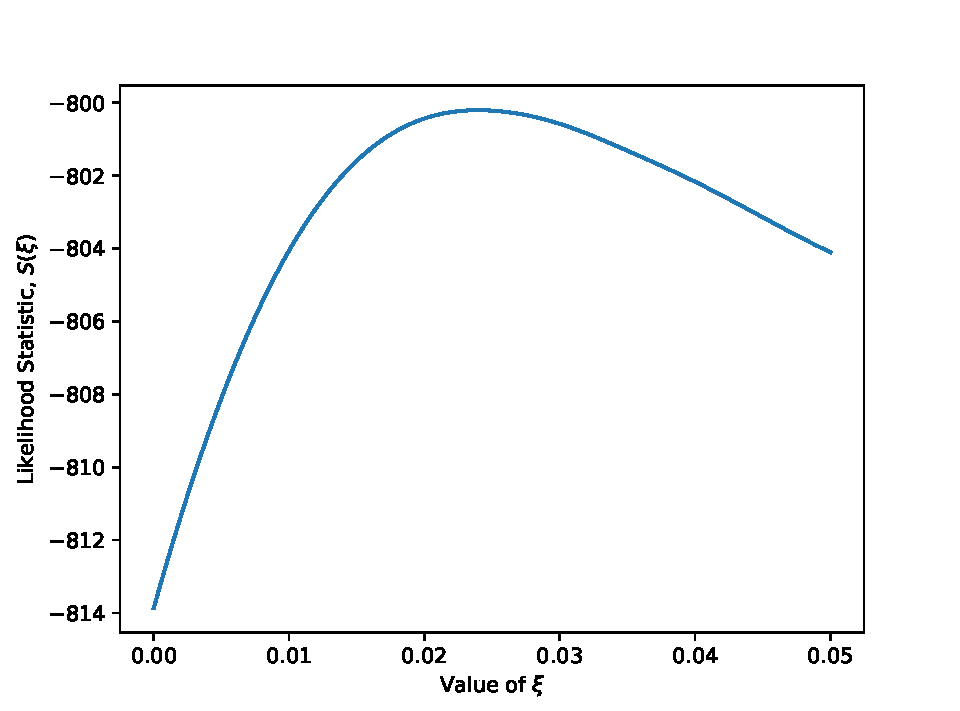
\includegraphics[width=1\textwidth]{{Figures/xi_plot.pdf}}
	\captionof{figure}{S($\xi$) vs $\xi$: The maximum occurs at $\xi = 0.024$.}
	\label{fig:play_by_play}
\end{figure}

\section{Dixon and Robinson}
Dixon and Robinson proposed an extension on the static Dixon and Coles model by incorporating the individual goal times.

\subsection{Model}
Dixon and Robinson began by 

It was clear that the Dixon and Coles model is more suitable for basketball and those team abilities will be used moving forward.
\section{Some Math Stuff}
The numbers can be seen in Table.  Using these numbers, and selecting the team with the highest probability of winning a game.  The accuracy of selecting a winner was 63.84\% and the value betting strategy won 57.84 units with 37.06\% winning bets.

Tried the Dixon and Coles model with a time parameter of 0.02 and the values seem more accurate.  The accuracy of selecting a winner was 63.21\% and the value betting strategy won 63.55 units with 38.03\% betting accuracy.  Did only the 2016 season and 64\% with the new vectorized way of doing it and 63.25 units.

Vectorized Dixon Coles and went from like 1341 seconds to 9 seconds for 3 seasons worth.  For some reason when I do Dixon Coles with the time factor with 2014, 2015 it gives me weird numbers but works perfectly fine with 2016 and 2017.  Must be something with the dataset
In the Dixon-Robinson model,.  By looking at NBA statistics the final minute of each quarter is likely to have an increase in scoring.


Dixon and Robinson model 1 is shown in Table \ref{table:dr_1_141516}.  The accuracy of selecting a winner was 60.28\% and the value betting strategy won 98.14 units with 37.31\% betting accuracy.

The issue with the betting is that it likes to bet on very high odds as the model computes probabilities differently.  Odds over 5 are usually bet.


\begin{equation}
    \lambda_k(t) = 
    \begin{cases}
        \rho_{1}\lambda_{xy}\lambda_{k} & \text{for }t \in (11/48, 12/48],\\
        \rho_{2}\lambda_{xy}\lambda_{k} & \text{for }t \in (23/48, 24/48],\\
        \rho_{3}\lambda_{xy}\lambda_{k} & \text{for }t \in (35/48, 36/48],\\
        \rho_{4}\lambda_{xy}\lambda_{k} & \text{for }t \in (47/48, 48/48],\\
        \lambda_{xy}\lambda_{k} & \text{otherwise}
\end{cases}
\end{equation}

The away rate is similar $\mu_k(t)$.



The optimal value is 0.024.

\section{Team Model}

Just like the model from Section a, with $n$ teams, the offence parameters $\{\alpha_1,\ldots,\alpha_n\}$ $\{\beta_1,\ldots,\beta_n\}$ $\gamma_h$ are to be estimated.  The following constraint is imposed due to the 

$$\frac{1}{n}\sum^{n}_{i=1}\alpha_i = 100$$

For the NBA, there are 30 teams, which gives a total of 61 parameters to be estimated.

\section{Player Model}